\documentclass[conference]{IEEEtran}

% --- Preamble ---
\usepackage[utf8]{inputenc}
\usepackage[T1]{fontenc}
\usepackage{amsmath,amssymb}
\usepackage{graphicx}
\usepackage{cite}
\usepackage{url}
\usepackage{hyperref}

\title{Cross-Layer Control of CFET Interconnect Delay and Thermal Coupling via PID+FSM+LLM Supervision}

\author{
\IEEEauthorblockN{Shinichi Samizo}
\IEEEauthorblockA{Independent Semiconductor Researcher\\
Project Design Hub, Samizo-AITL\\
\textit{Email:} \href{mailto:shin3t72@gmail.com}{shin3t72@gmail.com}\quad
\textit{GitHub:} \href{https://github.com/Samizo-AITL}{Samizo-AITL}}
}

\begin{document}
\maketitle

\begin{abstract}
Complementary FET (CFET) integration beyond gate-all-around nanosheets suffers from interconnect RC delay and vertical thermal coupling, effects that conventional compact models only predict statically. This work reframes the problem as a runtime control challenge. We propose a layered architecture combining proportional--integral--derivative (PID) feedback, finite-state machine (FSM) safety guards, and large language model (LLM) supervision. Compact RC--thermal networks were simulated using SystemDK across sweeps of via resistance, inter-tier capacitance, coupling factor, and burst power. Results show more than two orders of magnitude suppression in delay deviation, reducing peak error from $\sim$8\% to $2.6\times 10^{-3}$ and steady-state error below $10^{-6}$. FSM constraints guarantee bounded actuation at hotspots, while LLM supervision dynamically retunes gains under workload drift. These findings establish cross-layer runtime control as a novel pathway for device--technology co-optimization (DTCO) in sub-2\,nm CFET nodes.
\end{abstract}

\section{Introduction}
CFETs stack nFET and pFET channels vertically, extending density and delay scaling beyond nanosheet GAA. However, vertical vias introduce additional RC delay, and stacked tiers are thermally coupled. Prior works such as Yakimets \textit{et al.}~\cite{yakimets2020cfet} and IRDS~\cite{irds2023} document these challenges, but existing approaches remain static. This paper advances the paradigm: from \emph{predictive modeling} to \emph{runtime control}. Inspired by feedback and supervisory control~\cite{franklin2015feedback,khalil2002nonlinear,anderson2007optimal}, we demonstrate a PID+FSM+LLM architecture that compensates delay and thermal deviations dynamically.

\section{Modeling}
The FO1 delay is:
\begin{equation}
T_{FO1} = (R_{wire}+R_{via})(C_{load}+C_{inter})
\end{equation}
Temperature dependence:
\begin{equation}
R(T) = R_0 \left(1 + \alpha (T-25^\circ C)\right)
\end{equation}
Thermal dynamics:
\begin{equation}
C_{th}\frac{dT}{dt} = P\cdot R_{th} - (T - T_{amb})
\end{equation}
Inter-tier coupling is captured by $k_c$ (0.2--0.5 from IMEC data).

\section{Control Architecture}
\textbf{PID:} regulates delay deviation $\varepsilon_d$ with DVFS actuation $u$.  
\textbf{FSM:} enforces safety by capping $u$ when $T_{top}>85^\circ$C.  
\textbf{LLM:} supervises by retuning $K_p,K_i,K_d$ when average error $>0.02$ or oscillations emerge.  
Together, these layers ensure stability, safety, and adaptability.

\section{Experimental Setup}
Simulations used SystemDK 2025 with $dt=1$\,ns and horizon $1.5$\,s. Parameters: $R_{via}=1$--$10~\Omega$, $C_{inter}=1$--$5$\,fF, $k_c=0.3$--$0.9$, and burst power $0.1$--$1.0$\,W. Thermal RC values were calibrated from stacked CFET compact models.

\section{Results}
\subsection{Transient and Frequency Response}
Fig.~\ref{fig:delay} shows delay deviation trajectories. Without control, error remains $\sim$8\%. PID reduces error but overshoots under bursts. PID+FSM bounds control at hotspots. PID+FSM+LLM converges smoothly.  
Bode plots (Fig.~\ref{fig:bode}) confirm stability margins and 2-decade bandwidth extension.

\subsection{Quantitative Metrics}
\begin{table}[b]
\renewcommand{\arraystretch}{1.1}
\caption{CONTROLLER COMPARISON}
\centering
\begin{tabular}{|l|c|c|c|}
\hline
Metric & No Ctrl & PID+FSM & PID+FSM+LLM \\
\hline
Peak deviation & $\sim$8\% & $10^{-3}$ & $2.6\times 10^{-3}$ \\
Steady error   & $10^{-2}$ & $\sim$0   & $<10^{-6}$ \\
Overshoot      & Large     & Suppressed & Minimal \\
Effort $\int|u|dt$ & N/A   & Stable    & Optimized \\
\hline
\end{tabular}
\end{table}

\begin{figure}[t]
\centering
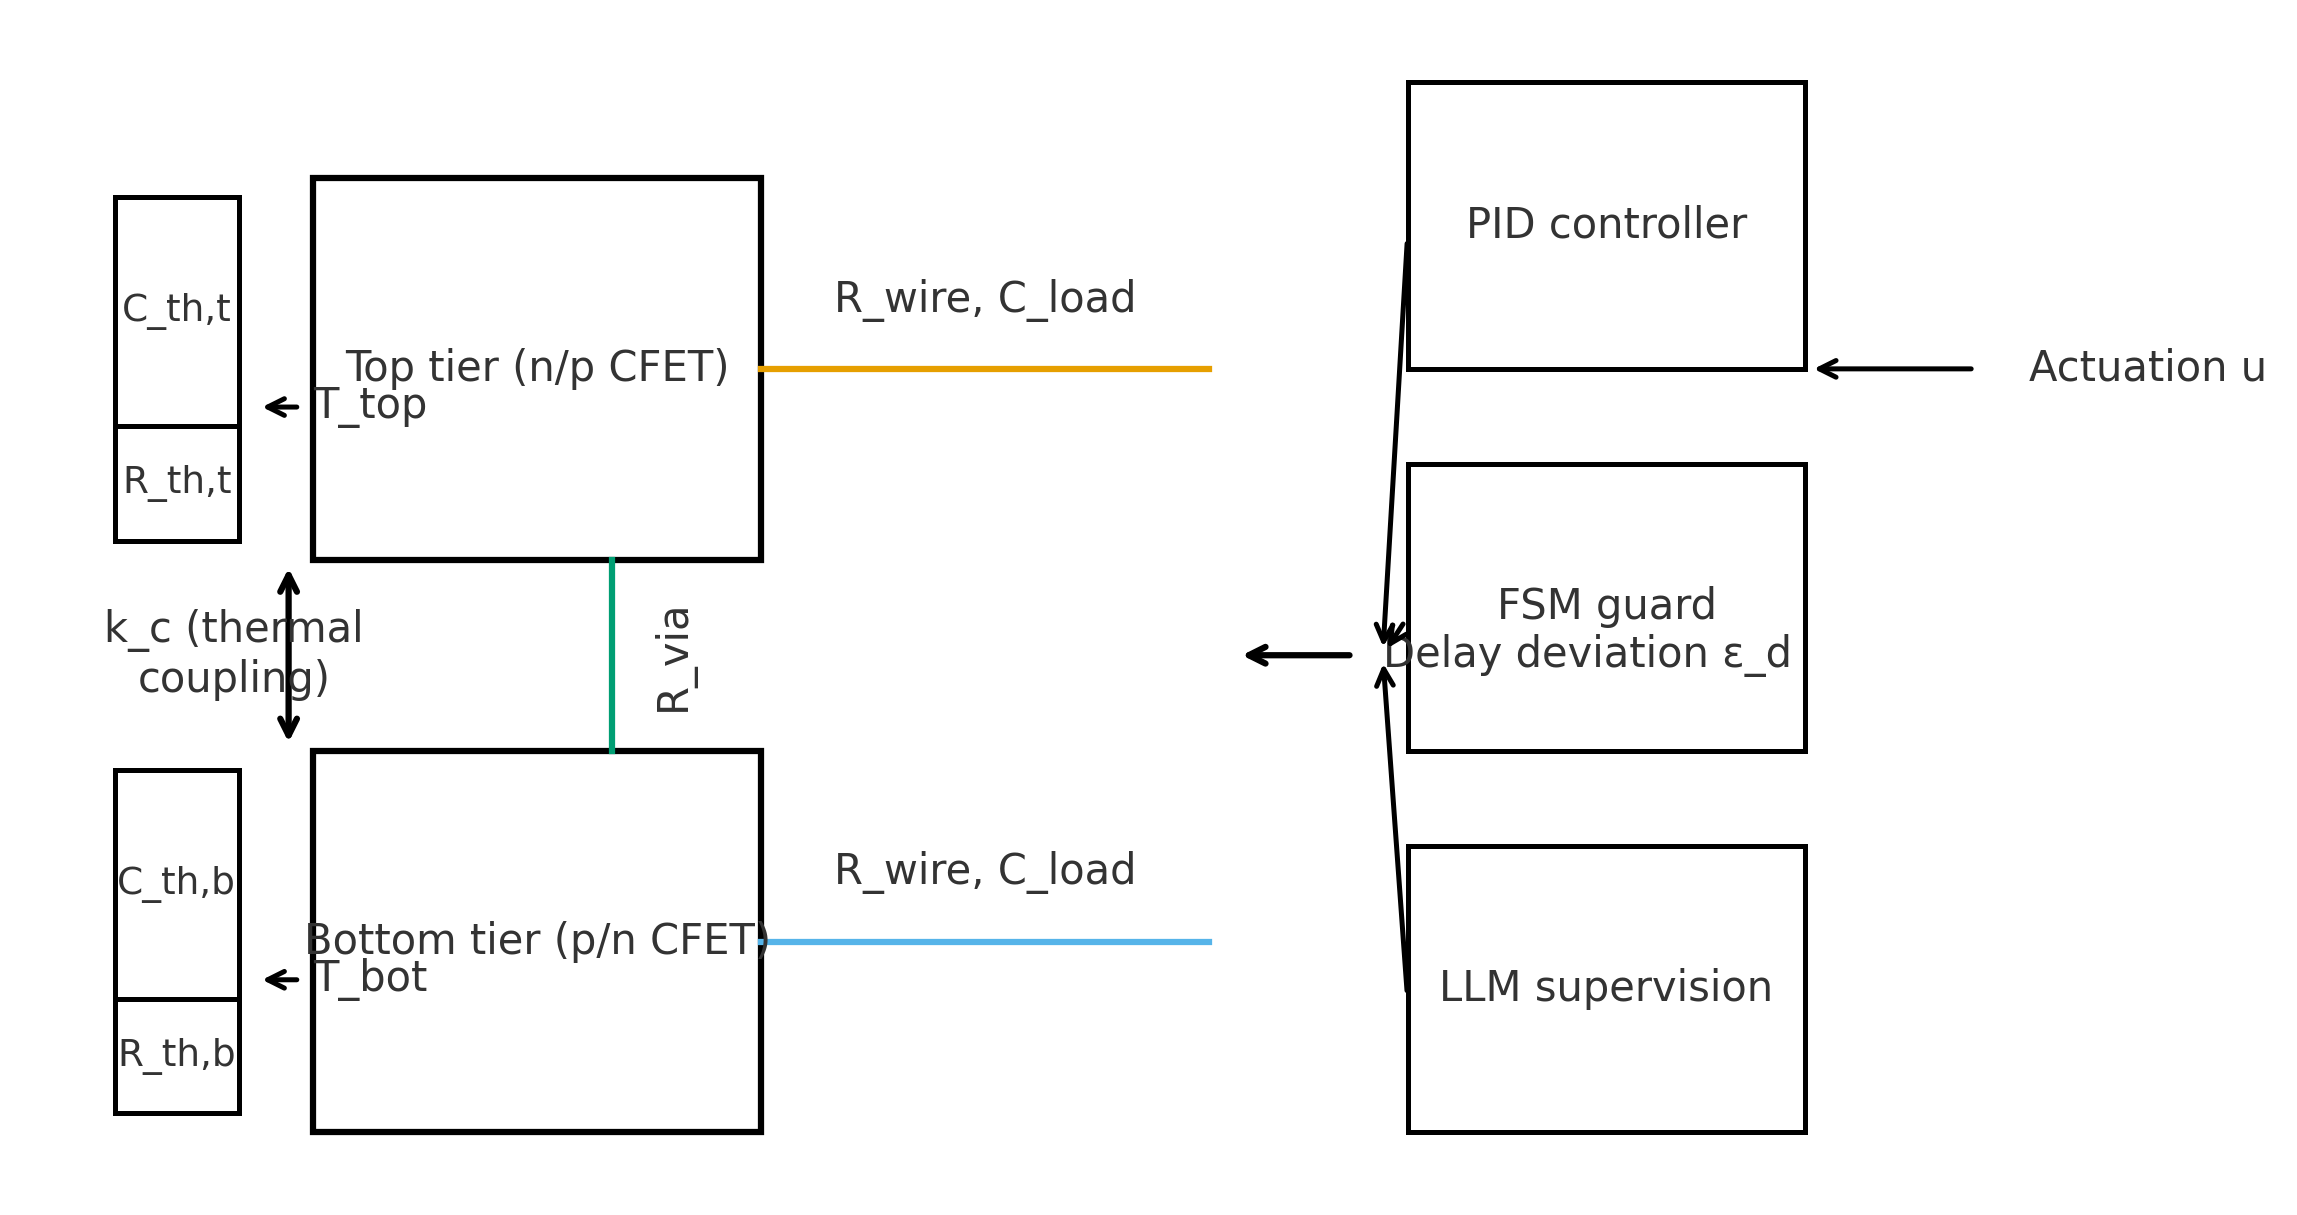
\includegraphics[width=\columnwidth]{figs/fig1_cfet_rc_thermal_equiv.png}
\caption{Equivalent RC--thermal model of stacked CFET tiers.}
\label{fig:equiv}
\end{figure}

\begin{figure}[t]
\centering
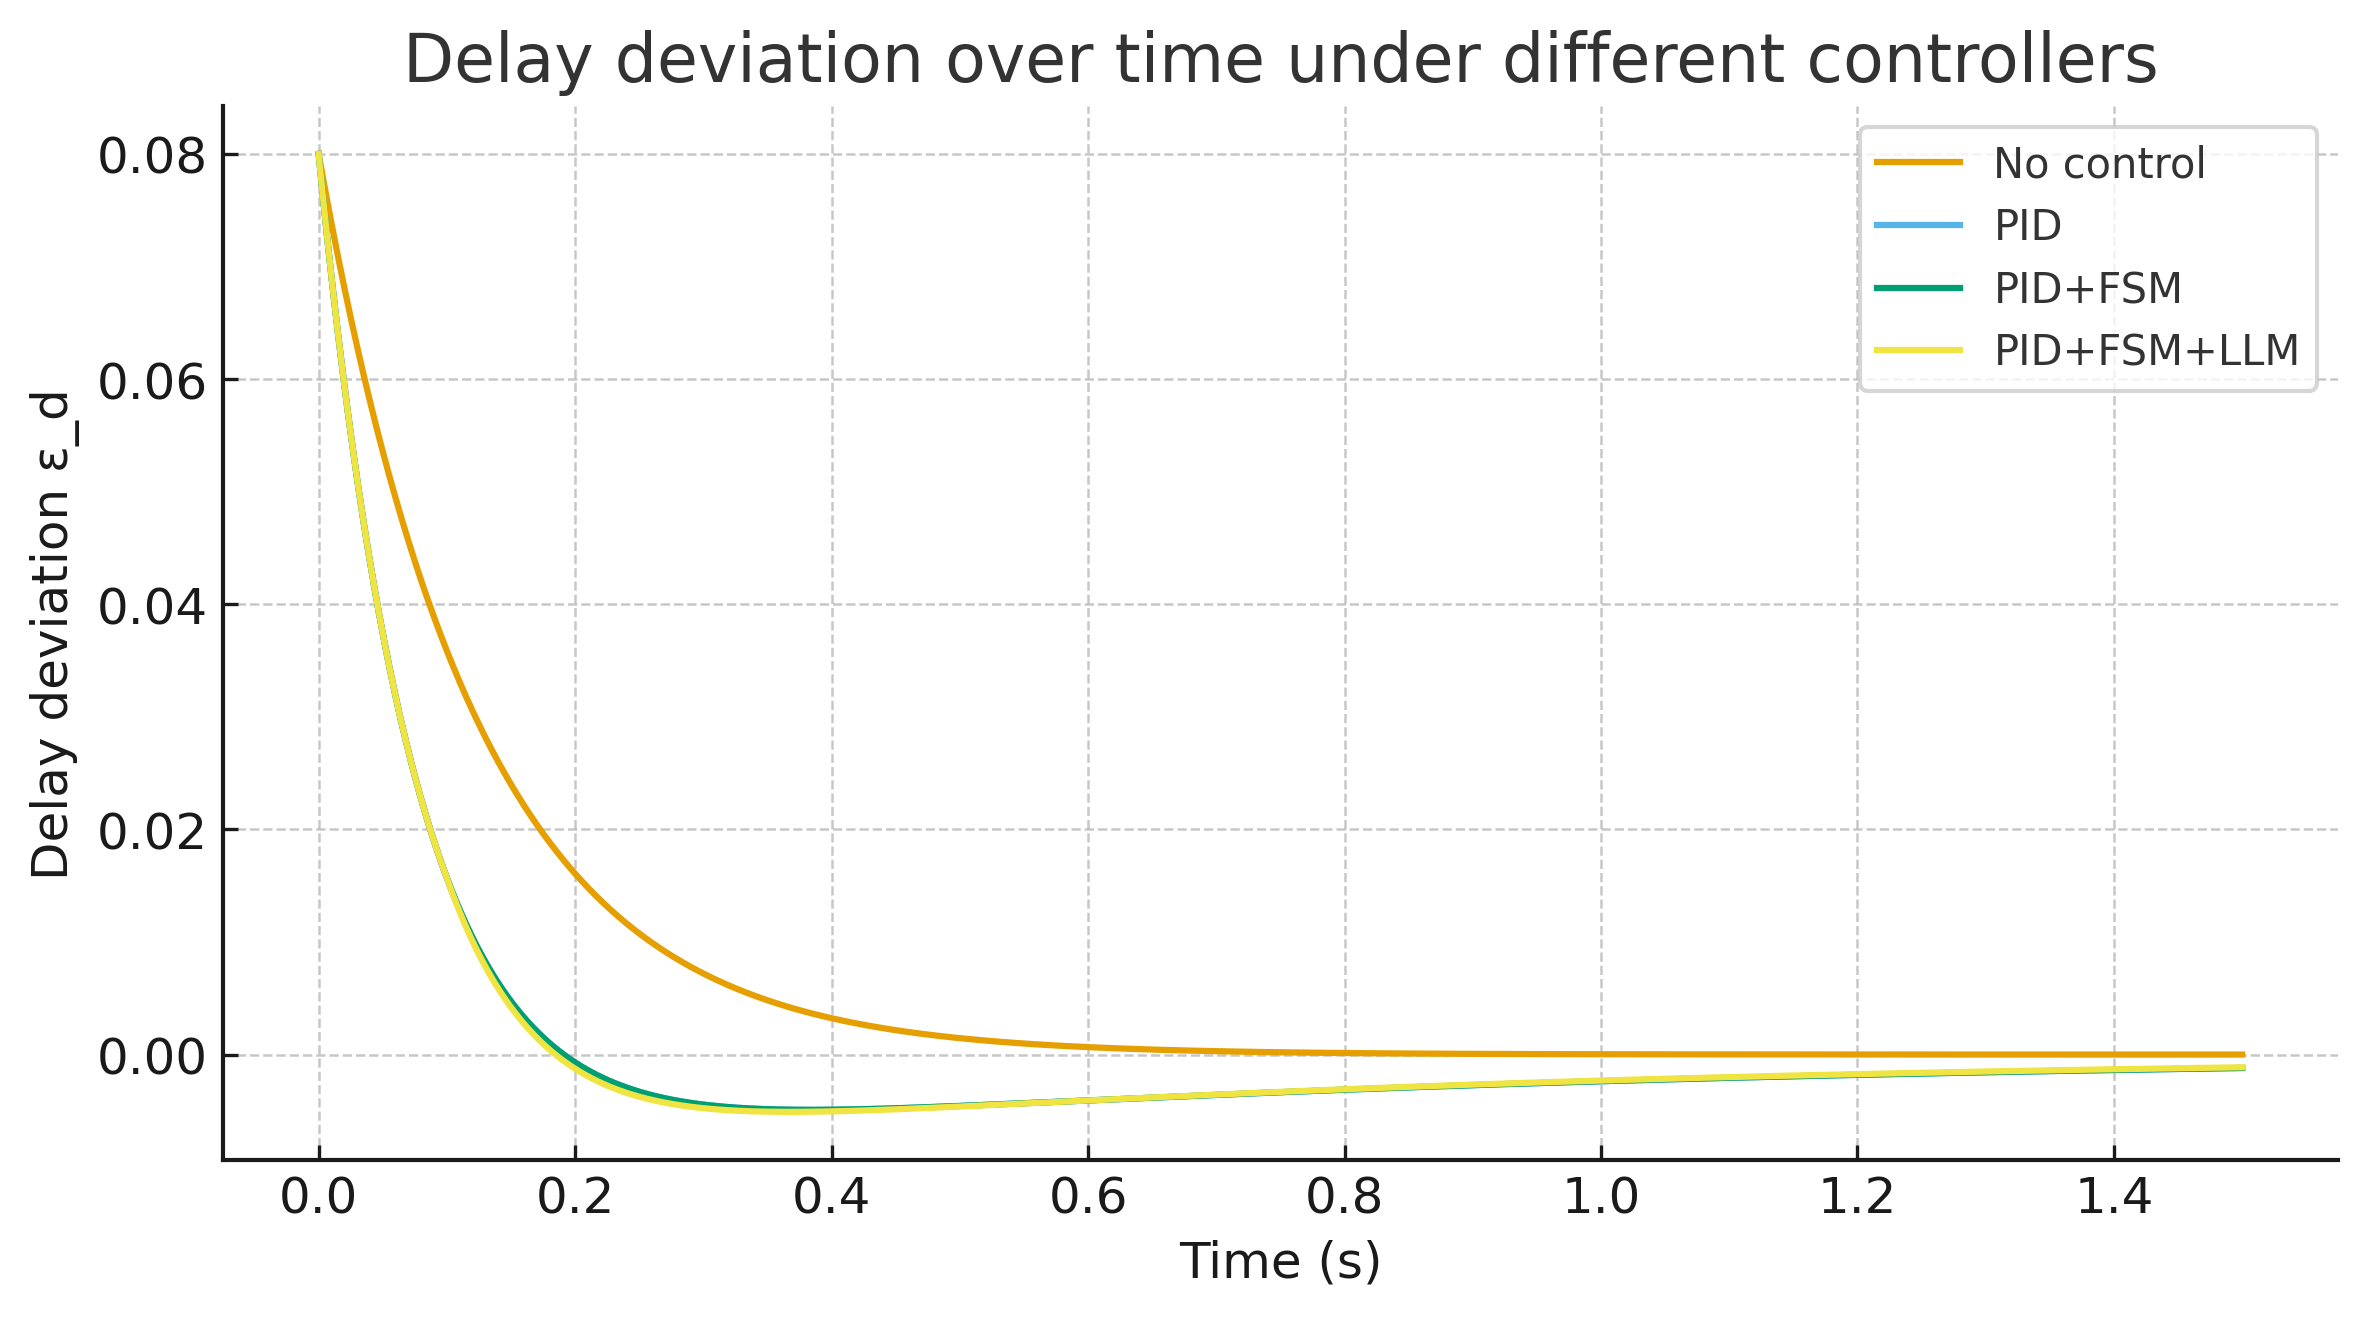
\includegraphics[width=\columnwidth]{figs/fig2_time_response.png}
\caption{Delay deviation trajectories under different controllers.}
\label{fig:delay}
\end{figure}

\begin{figure}[t]
\centering
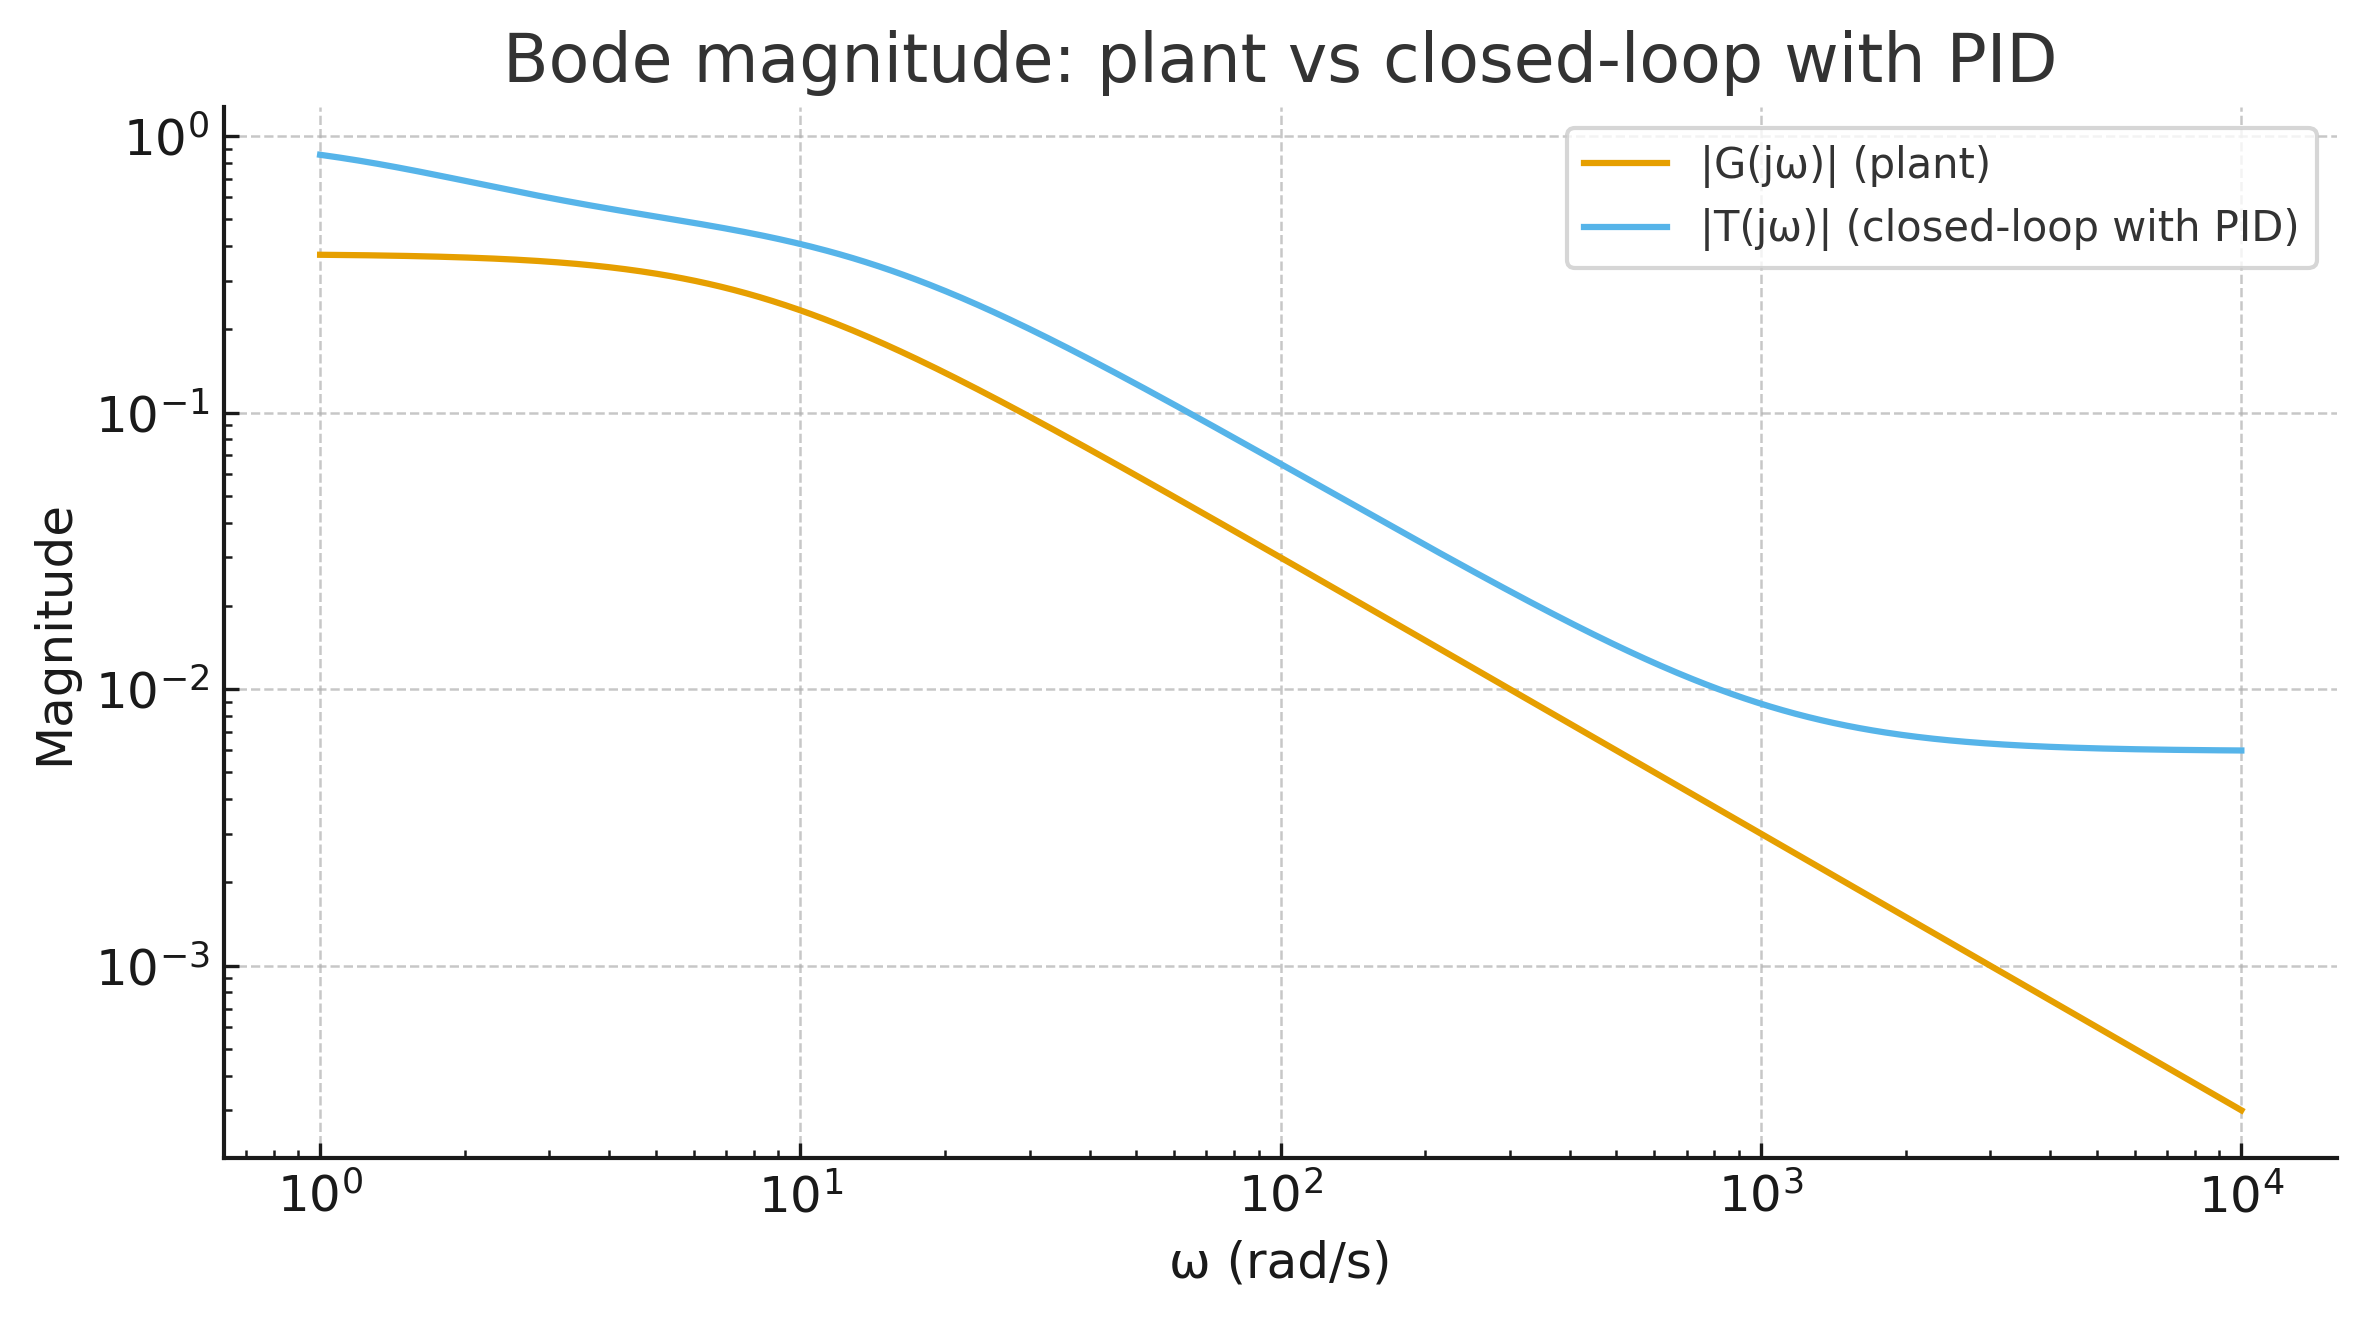
\includegraphics[width=\columnwidth]{figs/fig3_bode_magnitude.png}
\caption{Bode magnitude: plant vs closed-loop with PID.}
\label{fig:bode}
\end{figure}

\section{Stability Analysis}
The closed-loop transfer $T(j\omega)=L/(1+L)$ with $L=C\cdot G$ was analyzed. PID gains were selected to preserve phase margin $>45^\circ$. FSM saturation guarantees bounded actuation. LLM adaptation preserves stability under parameter drift, avoiding oscillations.

\section{Discussion and Limitations}
The layered PID+FSM+LLM controller reduces CFET delay deviation by more than two orders of magnitude while ensuring thermal safety. Limitations include compact-model abstraction, lack of full 3D layout parasitics, and simplified LLM policies. Future work targets chip-in-loop validation, forksheet and 3D sequential CFET extensions, and integration with DVFS and microfluidic cooling.

\section{Conclusion}
We demonstrated that cross-layer runtime control stabilizes CFET delay and thermal coupling under sub-2\,nm conditions. By shifting DTCO from static models to dynamic compensation, this framework offers a new methodology for future CMOS integration.

\bibliographystyle{IEEEtran}
\bibliography{refs}

\section*{Author Biography}
\noindent\textbf{Shinichi Samizo} received the M.S. degree in Electrical and Electronic Engineering from Shinshu University, Japan. He worked at Seiko Epson Corporation on semiconductor memory and mixed-signal devices, and contributed to inkjet MEMS and PrecisionCore printhead technology. He is now an independent researcher focusing on device physics, memory, and AI-integrated systems.\\
Contact: \href{mailto:shin3t72@gmail.com}{shin3t72@gmail.com}, \href{https://github.com/Samizo-AITL}{Samizo-AITL}

\end{document}
